\chapter{Конструкторская часть}
\section{IDEF0}
Концептуальная модель разрабатываемого компилятора в нотации IDEF0 представлена на рисунках \ref{img:2.2}.

\captionsetup{justification=centering,singlelinecheck=off}
\begin{figure}[h!]
	\centering
		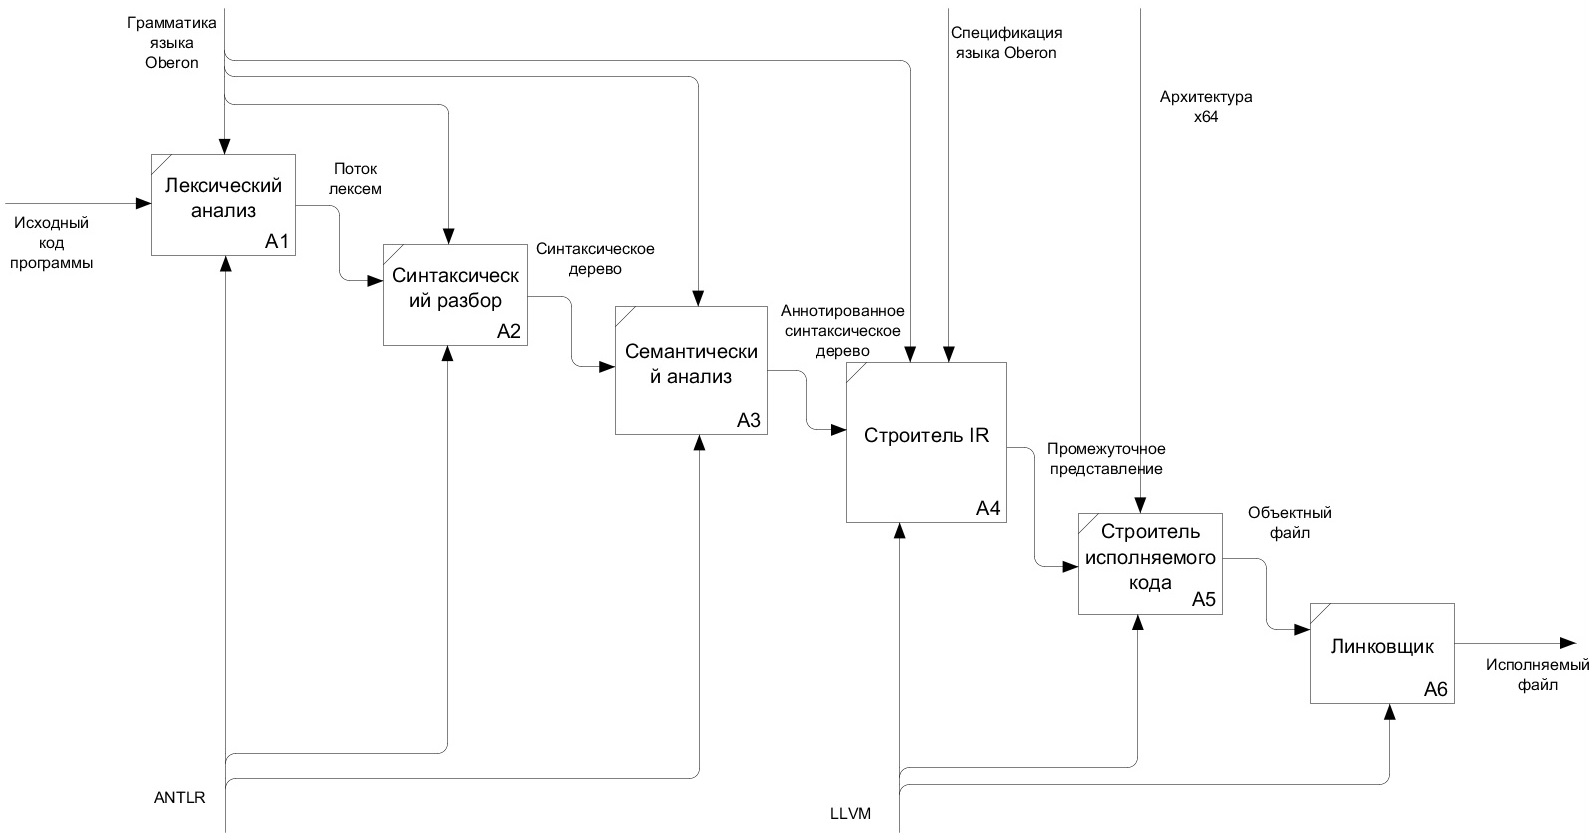
\includegraphics[,scale=0.]{./img/2.2.jpg}
		\caption{Концептуальная модель в нотации IDEF0 (A1-A6).}  
		\label{img:2.2}
\end{figure}
\section{Язык Oberon}
Oberon – язык программирования высокого уровня, предназначенный для исполнения программ на одноимённой операционной системе и основанный на таких языках, как Modula-2, Pascal.

Основные свойства и особенности языка Oberon:
\begin{itemize}[label = ---]
    \item \textbf{Простота и лаконичность}: Oberon известен своей минималистичной и лаконичной синтаксической структурой. Язык был разработан так, чтобы быть легким для восприятия и использования, что делает его подходящим как для обучения, так и для написания эффективного системного программного обеспечения.
    \item \textbf{Модульная структура}: Как и его предшественники, Oberon поддерживает модульную структуру программ. Модули являются основной единицей компиляции и разделения кода, что способствует разработке более структурированных и легко поддерживаемых программ.
    \item \textbf{Статическая типизация}: Oberon использует статическую типизацию, предоставляя компилятору полную информацию о типах данных во время компиляции. Это помогает обнаруживать ошибки типов на ранних этапах разработки и повышает надежность программ.
    \item \textbf{Поддержка системы типов и строгие проверки}: Язык обеспечивает строгую проверку типов, включая проверки на совместимость и преобразования типов. Это уменьшает количество ошибок времени выполнения и улучшает безопасность кода.
    \item \textbf{Ассоциация с операционной системой Oberon}: Язык тесно интегрирован с операционной системой Oberon, которая была разработана для демонстрации эффективного использования языка и его возможностей. Операционная система Oberon предоставляет среду, в которой программы на данном языке могут работать наиболее эффективно.
    \item \textbf{Гарвардская архитектура и интеграция с конкретным оборудованием}: Oberon был разработан с учетом особенностей гарвардской архитектуры, где программы и данные хранятся раздельно. Это помогает оптимизировать выполнение программ и использование памяти. Краткий пример кода на языке Oberon приведен в Листинге 10, где:
    \item MODULE HelloWorld; --- объявляет новый модуль с именем HelloWorld.
    \item IMPORT Out; --- импортирует модуль Out, который содержит процедуры для вывода текста.
    \item PROCEDURE Main*; --- объявляет основную процедуру Main, помеченную звездочкой, что означает, что эта процедура экспортируется и может быть вызвана извне.
    \item BEGIN ... END; --- определяет тело процедуры, в котором вызывается процедура Out.String для печати строки на экран, за которой следует вызов Out.Ln, который переводит
\end{itemize}

\begin{lstlisting}[label = 7, caption = Краткий пример кода на языке Oberon]
MODULE HelloWorld;
IMPORT Out;

PROCEDURE Main*;
BEGIN
Out.String("Hello, World!"); Out.Ln;
END Main;

END HelloWorld.
\end{lstlisting}

Грамматика языка Oberon формально описана в Приложении А и включает в себя правила синтаксиса для всех конструкций языка, таких как объявления модулей, процедур и типов данных. Этот раздел является ключом к пониманию внутренней структуры языка и его компиляции.

\section{Лексический и синтаксический анализаторы}
Лексический и синтаксический анализаторы в данной работе генерируются с помощью ANTLR. На вход поступает грамматика языка в формате ANTLR4 (файл с расширением .mod).

В результате работы создаются файлы, содержащие классы лексера и парсера, а также вспомогательные файлы и классы для их работы. Также генерируются шаблоны классов для обхода дерева разбора, которое получается в результате работы парсера.

На вход лексера подаётся текст программы, преобразованный в поток символов. На выходе получается поток токенов, который затем подаётся на вход парсера. Результатом его работы является дерево разбора.

Ошибки, возникающие в ходе работы лексера и парсера, выводятся в стандартный поток ввода-вывода.

\section{Семантический анализ}
Абстрактное синтаксическое дерево можно обойти двумя способами: применяя паттерн Listener или Visitor.

Listener позволяет обходить дерево в глубину и вызывает обработчики соответствующих событий при входе и выходе из узла дерева.

Visitor предоставляет возможность более гибко обходить построенное дерево и решить, какие узлы и в каком порядке нужно посетить. Таким образом, для каждого узла реализуется метод его посещения. Обход начинается с точки входа в программу (корневого узла).

\section*{Выводы}

В текущем разделе была представлена концептуальная модель в нотации IDEF0, приведена грамматика языка Oberon, описаны принципы работы лексического и синтаксического анализаторов и идея семантического анализа.